
Computerspiele werden Jahr für Jahr größer und aufwändiger. In den 70er-Jahren sind Spiele wie das ikonische Pong mit einfachster 2D-Grafik entwickelt worden. 
\begin{figure}
	\begin{subfigure}[b]{.49\textwidth}
		\centering
		\tikzset{external/export next=false}
		\begin{tikzpicture}
			\fill[black]  (0,0) rectangle (8,4.5);
		
			\fill[white]  (0.5,0.5) rectangle (.7,2);
			\fill[white]  (7.3,2) rectangle (7.5,3.5);
		
			\fill[white]  (5,2) rectangle (5.2,2.2);
		
			\draw[very thick,dashed,white] (4,0) -- (4,4.5);
		
			\fill[white]  (3.1,3.5) rectangle (3.5,4.2);
			\fill[black]  (3.2,3.6) rectangle (3.4,4.1);
		
			\fill[white]  (4.5,3.5) rectangle (4.9,4.2);
			\fill[black]  (4.6,3.6) rectangle (4.8,4.1);
			\end{tikzpicture}
		\subcaption{Nachbau der Grafik des 1972 erschienen Pong.}
	\end{subfigure}
	\begin{subfigure}[b]{.49\textwidth}
		\centering
		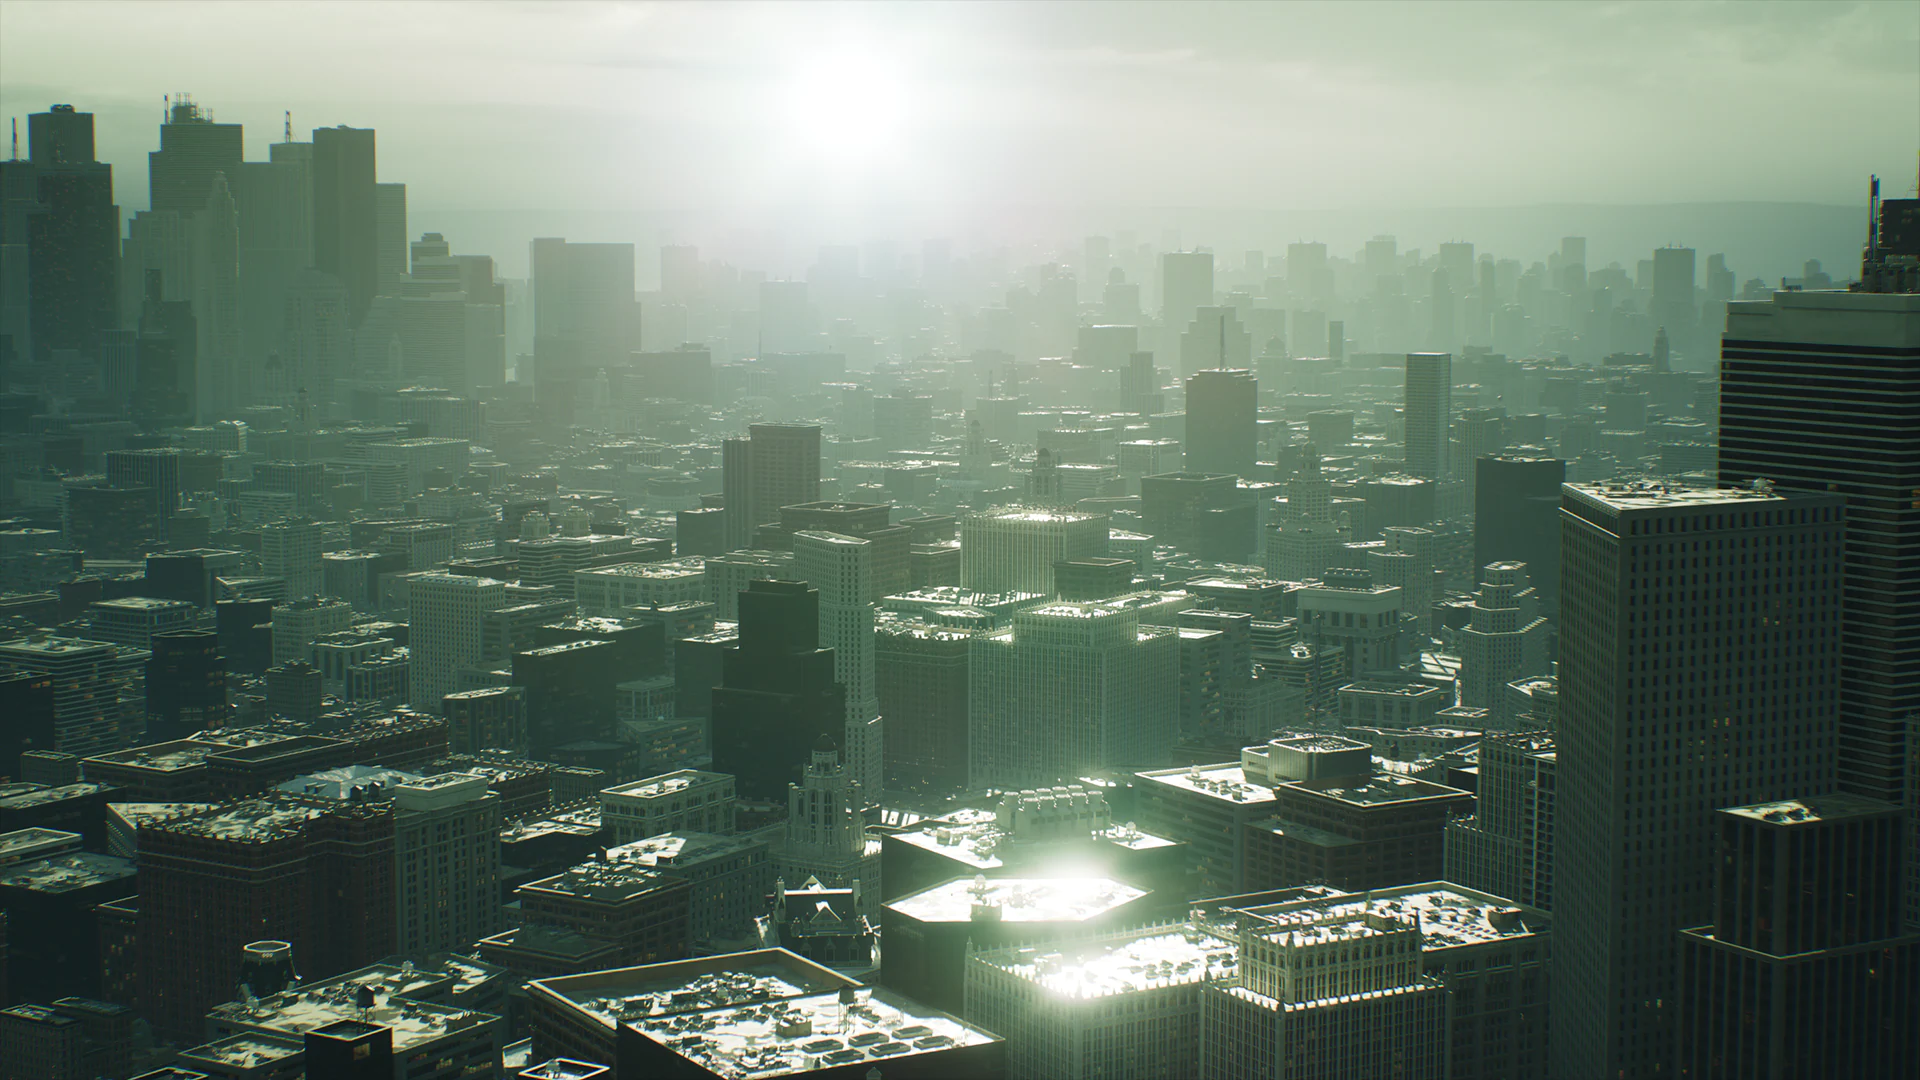
\includegraphics[height=4.5cm]{unreal-5.png}
		\subcaption{Unreal Engine 5 Technik-Beispiel\protect\footnotemark.}
	\end{subfigure}
	\caption{Vergleich der Computerspielgrafik von 1972 und 2022.}\label{fig:grafikvergleich}
\end{figure}
\footnotetext{\url{https://unrealengine.com/marketplace/en-US/learn/city-sample}}
Mit der Zeit wurden Spiele dann in 3D-Grafik entwickelt und erzeugen wie die 2022 erschienene Unreal~Engine~5~\cite{EpicGamesInc.} inzwischen teils von der Realität fast nicht mehr zu unterscheidende Bilder. In Abbildung~\ref{fig:grafikvergleich} wird die Entwicklung der Computerspielgrafik in letzten 50 Jahren veranschaulicht. Diese realistischere Grafik erfordert deutlich mehr Rechenleistung als simple Grafik und während die Rechenleistung der Computer in den letzten Jahrzehnten enorm gestiegen ist, wird seit einigen Jahren auch in der Computerspielindustrie stark auf Möglichkeiten der Leistungssteigerung durch Nebenläufigkeit gesetzt~\cite{Tatarchuk2014,Genova2015,Gyrling2015,Schott2016,Hodgman2016,White2018}.

\subsection{Die 3D-Spielebibliothek Blocklib}
Die Blocklib ist eine seit 2016 von Studierenden der Ostbayerischen Technischen Hochschule Regensburg entwickelte Spielebibliothek. Konzeptuell (und visuell, wie in Abbildung~\ref{fig:blocklibminecraft} zu sehen) ähnelt sie sehr dem 2011 offiziell erschienenen Spiel Minecraft~\cite{Mojang}.
\begin{figure}[!htbp]
	\begin{subfigure}[b]{.49\textwidth}
		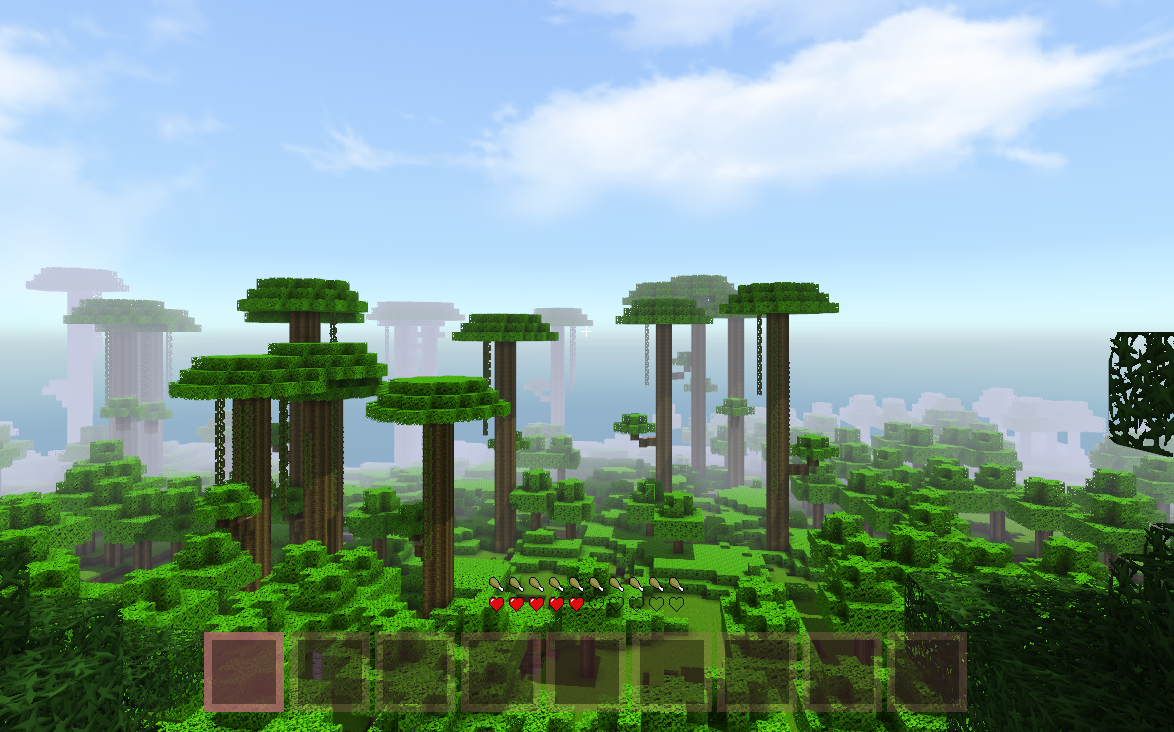
\includegraphics[width=\textwidth]{blocklib.png}
		\subcaption{Bildschirmfoto der Blocklib.}
	\end{subfigure}
	\begin{subfigure}[b]{.49\textwidth}
		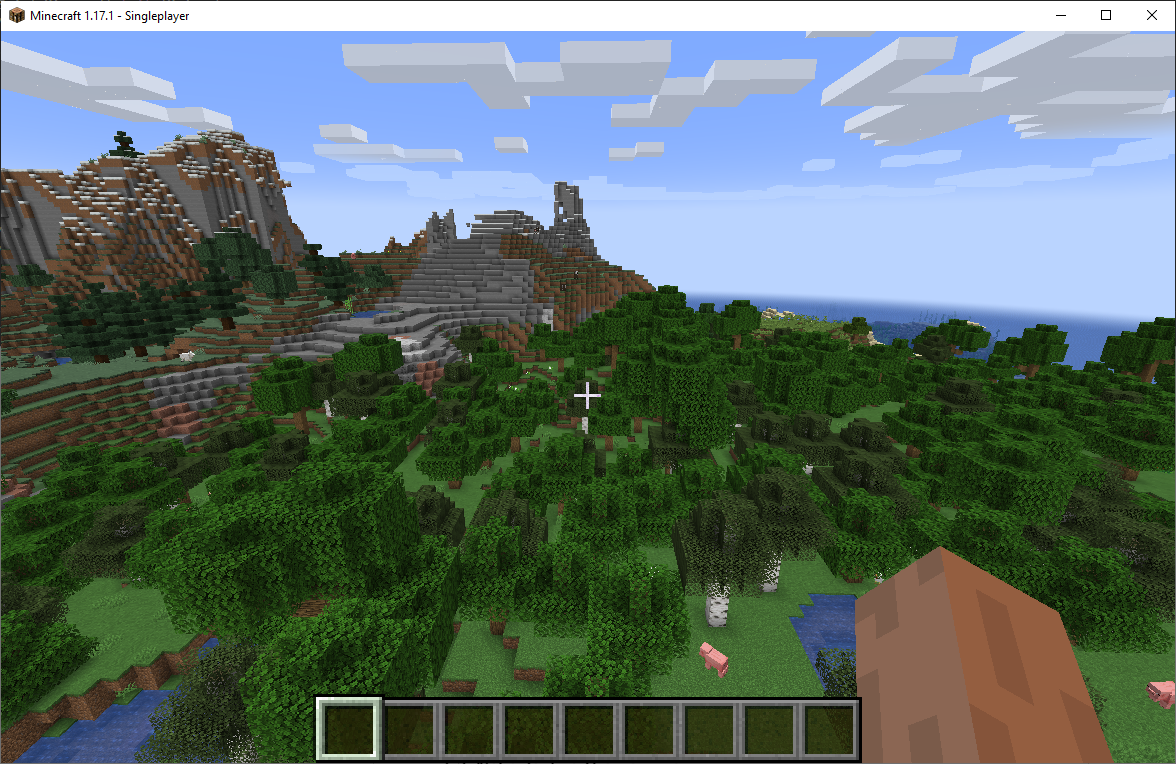
\includegraphics[width=\textwidth]{minecraft.png}
		\subcaption{Bildschirmfoto von Minecraft Version 1.17.1.}
	\end{subfigure}
	\caption{Bildschirmfotos der Blocklib und von Minecraft.}\label{fig:blocklibminecraft}
\end{figure}
Eines der Ziele bei der Entwicklung der Blocklib ist, Studierenden ein Werkzeug zu bieten, mit dem Studieninhalte verständlich vermittelt werden,  beispielsweise durch die Visualisierung der Verhaltensweise bestimmter Algorithmen~\cite{Helgert2018}. Des Weiteren bietet die Blocklib die Möglichkeit, selbst einfache Programme zu schreiben und durch die grafische Darstellung visuelles Feedback zu dem selbst entwickelten Code zu erhalten. Darüber hinaus ist die Blocklib eine Bibliothek, die in Projekten und Abschlussarbeiten in verschiedene Richtungen weiterentwickelt werden kann. So sind bereits Projekte in den Bereichen prozedurale Programmierung~\cite{Beer2017,Ebbinger2018a,Kalle2018,Sellner2020,Kohler2021}, maschinelles Lernen~\cite{Mayer2021}, künstliche Intelligenz~\cite{Amthor2017,Weidner2018,Bunke2021,Mayer2021}, Computergrafik~\cite{Zink2016,Ebbinger2018,Werner2018} und vielen weiteren durchgeführt worden, um die Blocklib zu erweitern.

Wie Minecraft zeichnet sich die Blocklib dadurch aus, dass die Welt aus einzelnen Blöcken besteht, von denen jeder einzeln hinzugefügt und entfernt werden kann. Die Welt in der Blocklib wird durch Algorithmen, man sagt auch \emph{prozedural}, generiert. Aufgrund dessen lässt sich die Welt in alle Richtungen beliebig weiter generieren und ist damit quasi beliebig groß. Deswegen kann die Welt nicht auf einmal vollständig generiert werden. Stattdessen wird sie in Bereiche fester Größe, sogenannte \emph{Chunks}, eingeteilt. Es werden dann nur die Chunks generiert, die sich in einer bestimmten Entfernung von der Kamera befinden.

Damit die Welt der Blocklib grafisch sichtbar wird, muss sie \emph{gerendert}, also gezeichnet, werden. Das lässt sich technisch auf verschiedene Arten lösen, in der Blocklib wird dafür auf die offene Grafikschnittstelle OpenGL~\cite{TheKhronosGroup,Vries2020} zurückgegriffen. Wie andere Spiele nutzt die Blocklib Nebenläufigkeit, um bestimmte Aufgaben wie das Generieren von Chunks schneller durchführen zu können. Bisher existieren allerdings, dynamisch gewachsen, viele verschiedene Ansätze, die nicht miteinander kooperieren. Dadurch ist es nötig, jedes Mal ein neues Konzept zu entwickeln, wenn Nebenläufigkeit genutzt werden soll. Zudem werden die Simulation der Spielebibliothek und das Rendering nicht nebenläufig ausgeführt. Das begrenzt die Geschwindigkeit der Blocklib im Vergleich zu dem Fall, dass die beiden Systeme parallel ausgeführt werden.

Ziel dieser Arbeit ist es daher, gängige Praktiken zur Nutzung von Nebenläufigkeit in der Spielindustrie zu analysieren und darauf aufbauend einen Entwurf für eine nebenläufige Architektur in der Blocklib zu konzipieren. Des Weiteren soll die Architektur implementiert und in das bestehende Ökosystem der Blocklib integriert werden. Die so entstandene Architektur soll zudem, bezogen auf die Leistung, mit der vorherigen Architektur verglichen werden.

In der folgenden Arbeit werden dafür zunächst in Kapitel~\ref{kap:grundlagen} einige Grundlagen und Begriffe eingeführt und typische nebenläufige Architekturen in der Spielindustrie beleuchtet. In Kapitel~\ref{kap:entwurf} wird die Analyse der Blocklib und der daraus resultierende Entwurf für die nebenläufige Architektur beschrieben. Danach beschreibt Kapitel~\ref{kap:Implementierung} die Details der Implementierung der Architektur und wie diese in die Blocklib integriert wird. In der Performanceanalyse in Kapitel~\ref{kap:performance} werden die Leistung der neuen und der alten Architektur verglichen, indem Messungen von verschiedenen Leistungsindikatoren in mehreren Szenarien analysiert und bewertet werden. In den Kapiteln~\ref{kap:Fazit} und \ref{kap:ausblick} werden Ergebnis und Erfolg der Arbeit erörtert und schließlich ein Ausblick auf verschiedene Themen gegeben, die in Zukunft bearbeitet werden können.